\chapter{Appendix: Simulation Depth Camera Misalignment}\label{sec:appendix:gz_depth_camera}

When first attempting to implement a depth camera as ground truth I noticed a misalignment of the depth camera FOV and a normal camera's image. This was the case even with equal camera parameters:


\begin{figure}[ht]
    \centering
    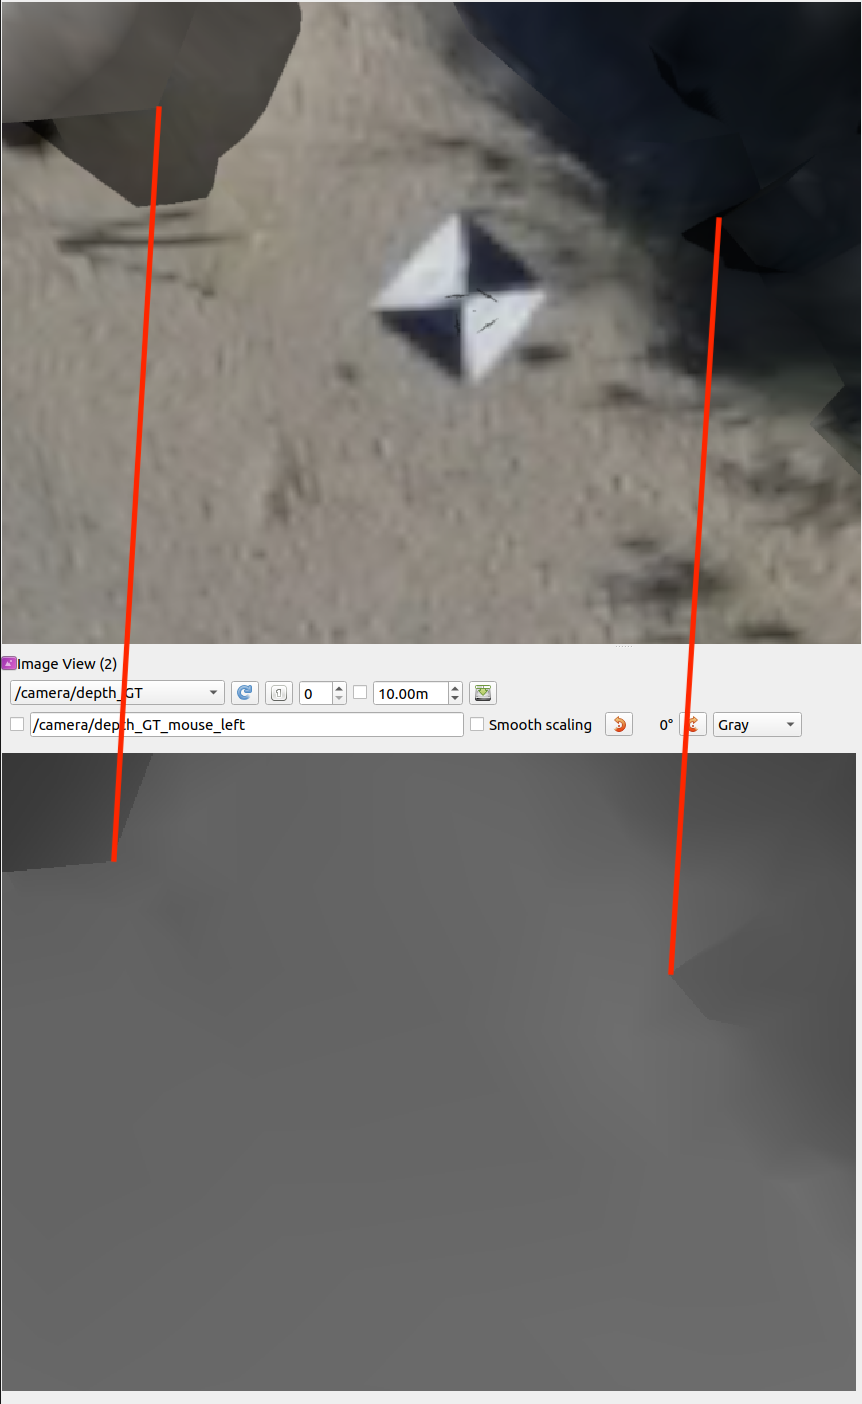
\includegraphics[scale=0.4]{images/appendix/GT_error/GT_image.png}
    \caption{Depth camera misalignment. Top: reference camera image of the stereo pair, Bottom: depth camera image}
    \label{fig:GT_error_sim}
\end{figure}
% \begin{figure}
%     \centering
%     
\includegraphics[scale=0.4]{images/stereo_camera_depth/GT_error_GT.png}
%     \caption{GT depth image with wrong calibration}
%     \label{fig:GT_error_GT} %TODO Use color coded image
% \end{figure}


Looking at \cref{fig:GT_error_sim}, we can see a misalignment of the depth camera's field of view and the normal reference camera at the same location with the same parameters. Later tests showed that there was an actual error in the Gazebo Garden source code. No matter what camera parameters were passed, the depth camera had the same FOV. 

Thanks to my friend and colleague Simone Nascivera, this bug could be fixed.